% Kron reduction / star-mesh transform: eliminating the phi node turns the
% ideal star (C^ext) into the fully-connected ambipolar mesh (C^amb).
% Capacitor halves coloured by species; phi is black.
\documentclass[tikz, border=4pt]{standalone}
\usepackage[american]{circuitikz}
\usetikzlibrary{calc}

\definecolor{spA}{HTML}{377EB8} % electron
\definecolor{spB}{HTML}{E41A1C} % lithium
\definecolor{spC}{HTML}{80B030} % chloride
\definecolor{spD}{HTML}{8A4FA0} % oxide
\definecolor{spE}{HTML}{E6AB02} % silver

\newcommand{\bicap}[5][]{% [style] A B cA cB
  \path (#2) -- (#3) coordinate[midway] (bcM);
  \begin{scope}
    \pgfinterruptboundingbox
    \clip let \p1=(#2), \p2=(#3), \n1={atan2(\y2-\y1,\x2-\x1)} in
      [rotate around={\n1:(bcM)}] ($(bcM)+(-6,-6)$) rectangle ($(bcM)+(0,6)$);
    \endpgfinterruptboundingbox
    \draw[#1,#4] (#2) to[C] (#3);
  \end{scope}
  \begin{scope}
    \pgfinterruptboundingbox
    \clip let \p1=(#2), \p2=(#3), \n1={atan2(\y2-\y1,\x2-\x1)} in
      [rotate around={\n1:(bcM)}] ($(bcM)+(0,-6)$) rectangle ($(bcM)+(6,6)$);
    \endpgfinterruptboundingbox
    \draw[#1,#5] (#2) to[C] (#3);
  \end{scope}
}

\begin{document}
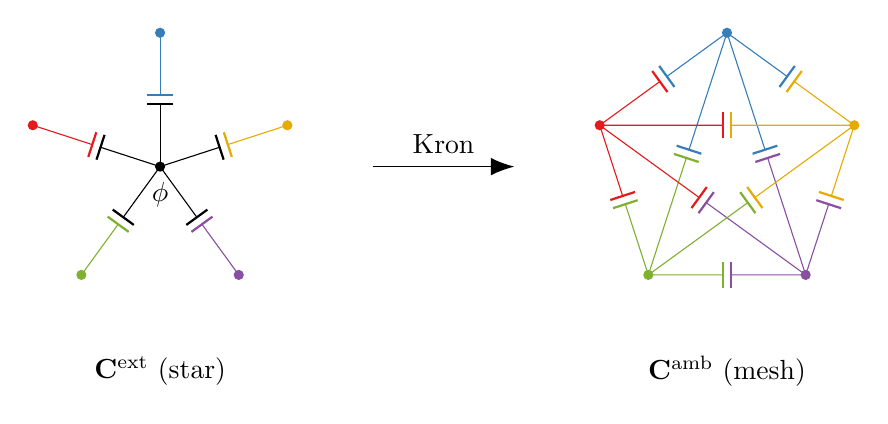
\begin{tikzpicture}
  \ctikzset{bipoles/length=0.55cm}
  \def\rad{1.7}

  % ---- left: star (with central phi) ----
  \begin{scope}[shift={(0,0)}]
    \coordinate (C) at (0,0);
    \foreach \i/\c in {1/spA, 2/spB, 3/spC, 4/spD, 5/spE} {
      \coordinate (L\i) at ({72 * (\i - 1) + 90}: \rad);
      \node[circle, fill=\c, inner sep=1.3pt] at (L\i) {};
    }
    \bicap{L1}{C}{spA}{black}
    \bicap{L2}{C}{spB}{black}
    \bicap{L3}{C}{spC}{black}
    \bicap{L4}{C}{spD}{black}
    \bicap{L5}{C}{spE}{black}
    \node[circle, fill=black, inner sep=1.3pt, label={[label distance=0pt]-90:$\phi$}] at (C) {};
    \node at (0,-2.6) {$\mathbf{C}^{\mathrm{ext}}$ (star)};
  \end{scope}

  % ---- arrow ----
  \draw[-{Latex[length=3mm]}, line width=0.6pt] (2.7,0) -- (4.5,0)
    node[midway, above=1pt] {Kron};

  % ---- right: mesh (phi eliminated) ----
  \begin{scope}[shift={(7.2,0)}]
    \foreach \i/\c in {1/spA, 2/spB, 3/spC, 4/spD, 5/spE} {
      \coordinate (R\i) at ({72 * (\i - 1) + 90}: \rad);
      \node[circle, fill=\c, inner sep=1.3pt] at (R\i) {};
    }
    \bicap{R1}{R2}{spA}{spB}
    \bicap{R1}{R3}{spA}{spC}
    \bicap{R1}{R4}{spA}{spD}
    \bicap{R1}{R5}{spA}{spE}
    \bicap{R2}{R3}{spB}{spC}
    \bicap{R2}{R4}{spB}{spD}
    \bicap{R2}{R5}{spB}{spE}
    \bicap{R3}{R4}{spC}{spD}
    \bicap{R3}{R5}{spC}{spE}
    \bicap{R4}{R5}{spD}{spE}
    \node at (0,-2.6) {$\mathbf{C}^{\mathrm{amb}}$ (mesh)};
  \end{scope}
\end{tikzpicture}
\end{document}
